% figure: 自控-教材例6-3PID结构图.png
% 用途：自控 06-2 —— 教材例6-3 的 PID 控制系统结构图（图 6-20）
% 构建：..\build.ps1 -File .\block-pid-6-3.tex
% 说明：旧图是教材页扫描，带页眉页脚与"图 6-20"题注、纹理发灰；本图按结构重画，
%       只保留系统本身。注意：原图 PID 块写作 K_p(1+1/(T_i s)+T_d s)，
%       其中 1/(T_i s) 在一行内会被读成 T_i s 的倒数的一半，本图改为 T_i s 项写成
%       \dfrac{1}{T_i s} 并分行，避免歧义。
\documentclass[border=10pt]{standalone}
\usepackage{fontspec}
\setmainfont{Cambria}
\usepackage{unicode-math}
\setmathfont{Cambria Math}
\usepackage{tikz}
\usetikzlibrary{positioning, arrows.meta, calc}
\usepackage{ctex}

\definecolor{figink}{HTML}{1E2228}
\definecolor{figsub}{HTML}{606874}
\definecolor{figfill}{HTML}{E8EFF8}

\begin{document}
\begin{tikzpicture}[
  x=1cm, y=1cm,
  line width=0.95pt, line cap=round, line join=round,
  >=Stealth,
  blk/.style = {draw=figink, line width=0.95pt, fill=figfill,
                minimum height=1.15cm, inner sep=4pt,
                anchor=center, font=\small},
  sum/.style = {draw=figink, line width=0.95pt, circle, inner sep=0pt,
                minimum size=0.42cm, anchor=center},
  sig/.style = {font=\small, color=figink, fill=white},
  lbl/.style = {font=\small, inner sep=1.5pt, fill=white}
]

\node[sum] (s1) at (0,0) {};
\node[blk, minimum width=2.9cm] (pid) at (2.6,0)
  {$K_p\left(1+\dfrac{1}{T_i s}+T_d s\right)$};
\node[blk, minimum width=2.6cm] (g) at (6.2,0)
  {$\dfrac{K}{s(s+1)(s+20)}$};

\draw[->] (-2.2,0) -- node[sig, above] {$R(s)$} (s1.west);
\draw[->] (s1.east) -- node[sig, above] {$E(s)$} (pid.west);
\draw[->] (pid.east) -- (g.west);
\draw[->] (g.east) -- node[sig, above] {$C(s)$} (8.6,0);
\draw[->] (7.6,0) -- (7.6,-1.9) -- (0,-1.9) -- (s1.south);

\node[lbl] at (-0.36,0.32) {$+$};
\node[lbl] at (-0.46,-0.32) {$-$};

\end{tikzpicture}
\end{document}
